\documentclass[12pt, a4paper]{article}

% ******************************** PACKAGE ****************************
\usepackage[top=1.5cm, bottom=1.5cm, left=1.5cm, right=1.5cm]{geometry}
\usepackage{amsmath}
\usepackage{amsmath}
\usepackage{amssymb}
\usepackage{enumitem}
\usepackage{fancyhdr}
\pagestyle{fancy}
\usepackage{tikz}
\usepackage{adjustbox}
\usepackage[colorlinks=true]{hyperref}
\usepackage{lastpage}

% ******************************** SETUP ********************************
\pagestyle{fancy}
\fancyhf{}
\fancyfoot[R]{\textit{\textbf{Andrea Savastano}}}

% *************************** MAIN PAGE INFO *****************************

% ******************************** DOCUMENTO ****************************
\begin{document}
	\section*{Prestazioni trasmissione Tecniche Diversità}
	
	\begin{adjustbox}{width=.95\paperwidth, center}
		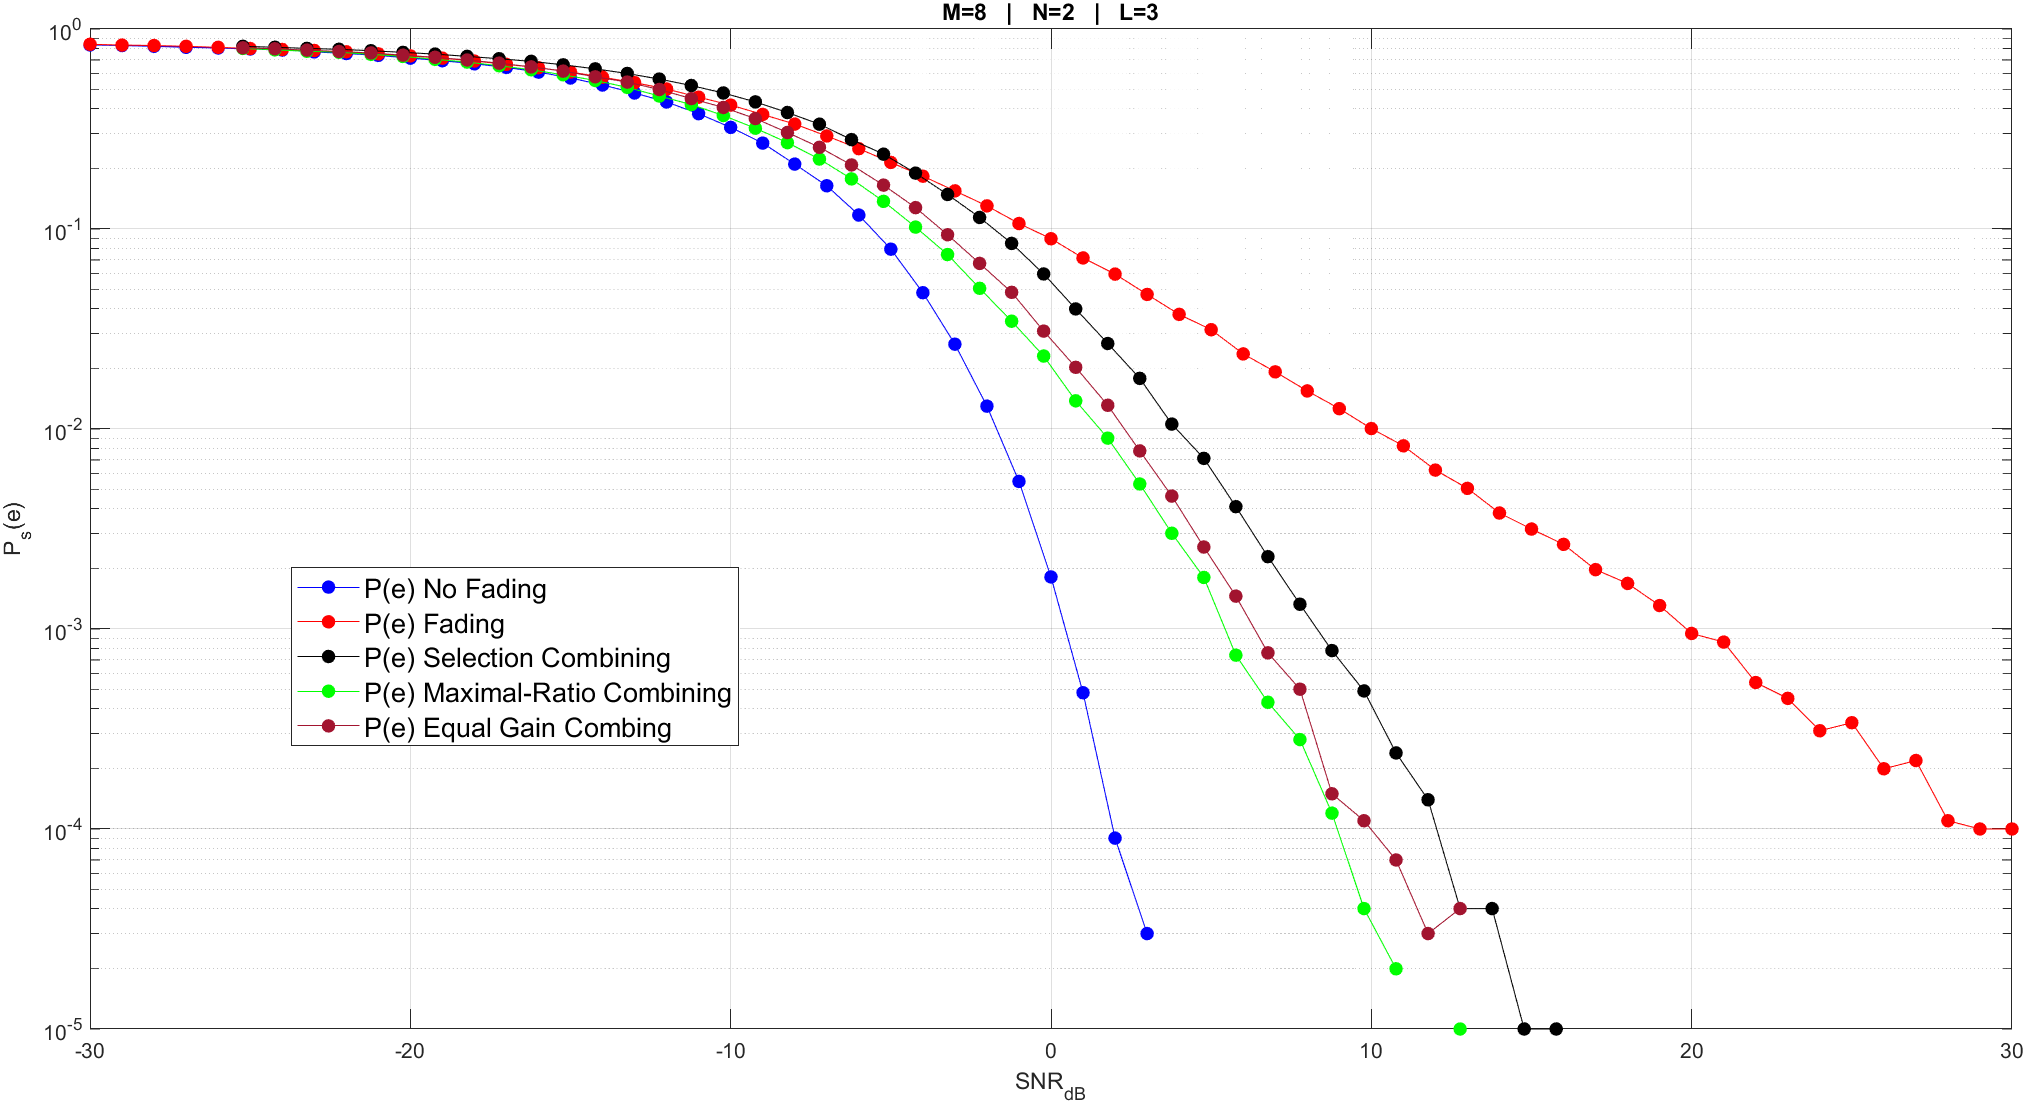
\includegraphics{images/untitled1.png}
	\end{adjustbox}\\\\
	La modulazione scelta per la simulazione di trasmissione è 8-PSK con \(L=3\) ritrasmissioni per le tre tecniche di diversità.\\
	Le cinque prestazioni graficate con diversi colori sono relative ad una trasmissione con rumore AWGN con \(N_0=1\) e \(MC=1\cdot10^5\) prove montecarlo.\\
	Tuttavia solo il grafico blu rappresenta le prestazioni in assenza di fading, mentre le restanti 4 prevedono un fading di Rayleigh:\\
	\[
	r=\alpha\cdot s+n, \,\,
	\begin{cases}
		\alpha\sim \text{Rayleigh}\\
		n\sim \mathcal{N}(0,\frac{N_0}{2})		
	\end{cases}
	\]\[
	\text{PDF della v.a. di Rayleigh: }\, f_R(r)=
	\begin{cases}
		\frac{r}{\sigma_R^2}e^{-r^2/(2\sigma_R^2)}, \, r\ge0\\
		0, \, r<0		
	\end{cases}
	\]
	
\end{document}